\section{Additional Results}
\label{sec:appendix_results}

\subsection{ImageNet-Scale Validation}

\begin{table}[h]
\centering\small
\caption{%
  ImageNet-scale replication. ResNet-50 (torchvision pretrained, $\sim76\%$ top-1), ImageNet-C severity 5, NINCO OOD, $n=30$ batches per cell.
  All 8 cells: $\DeltaA(\idonly) > \DeltaA(\mixed)$, $p < 0.05$.
  TENT gap exceeds ETA gap in every row, consistent with ETA's entropy threshold providing partial OOD gradient filtering.
}
\label{tab:imagenet_scale_app}
\begin{tabular}{llcrrr}
\toprule
Corruption & Method & $\alpha$ & ID-Oracle $\DeltaA$ & Mixed-Adapt $\DeltaA$ & paired $p$ \\
\midrule
fog & ETA  & 0.5 & $+0.059$ & $-0.004$ & $8.9 \times 10^{-12}$ \\
    & ETA  & 0.9 & $+0.045$ & $-0.018$ & $8.6 \times 10^{-7}$ \\
    & TENT & 0.5 & $+0.246$ & $+0.056$ & $5.8 \times 10^{-16}$ \\
    & TENT & 0.9 & $+0.273$ & $-0.079$ & $8.0 \times 10^{-15}$ \\
\midrule
jpeg & ETA  & 0.5 & $+0.050$ & $-0.025$ & $9.7 \times 10^{-13}$ \\
     & ETA  & 0.9 & $+0.011$ & $-0.020$ & $5.3 \times 10^{-4}$ \\
     & TENT & 0.5 & $+0.300$ & $+0.051$ & $1.5 \times 10^{-18}$ \\
     & TENT & 0.9 & $+0.386$ & $-0.012$ & $1.1 \times 10^{-18}$ \\
\bottomrule
\end{tabular}
\end{table}

\subsection{Streaming Validation}

\begin{figure}[h]
  \centering
  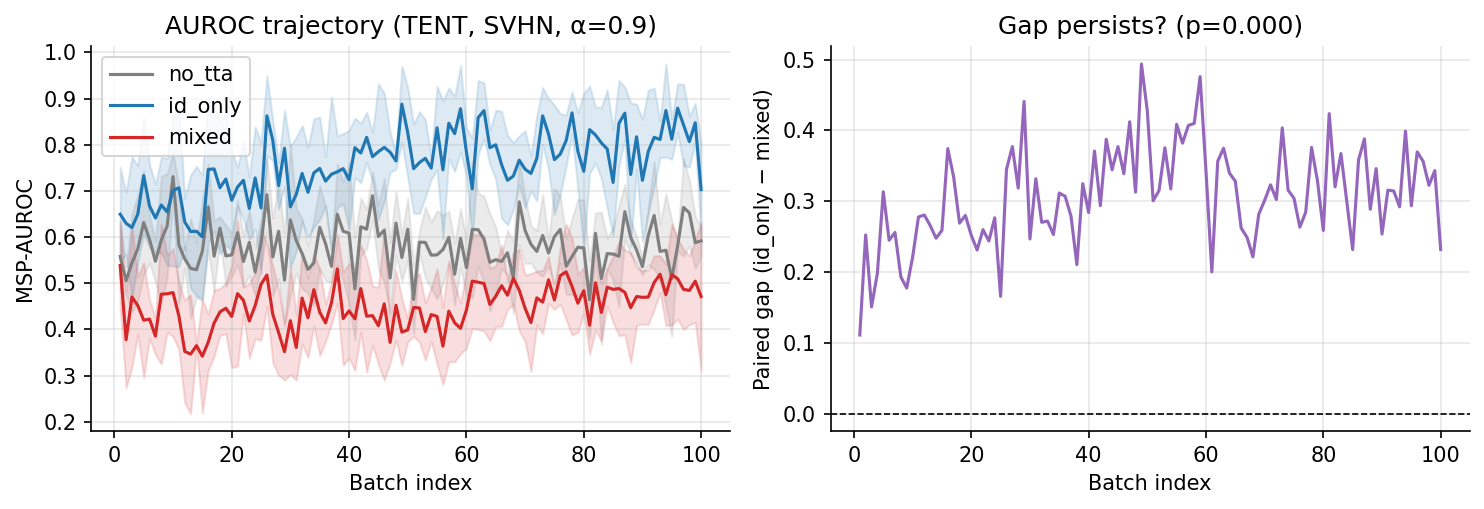
\includegraphics[width=\linewidth]{figures/fig_streaming.png}
  \caption{%
    \textbf{AUROC trajectory over 100 sequential batches without model reset (TENT, SVHN, $\alpha{=}0.9$, gaussian noise, 5 seeds).}
    \emph{Left}: MSP-AUROC per batch. ID-Oracle (blue) consistently exceeds Mixed-Adapt (red).
    \emph{Right}: Paired gap per batch. The gap persists without systematic decay---the contamination cost is not a single-batch artifact.
  }
  \label{fig:streaming}
\end{figure}

\begin{table}[h]
\centering\small
\caption{%
  Streaming validation: time-averaged MSP-AUROC over 100 sequential batches (no model reset).
  Paired gap $=$ ID-Oracle AUROC $-$ Mixed-Adapt AUROC, averaged over stream.
  8/8 cells significant ($p < 0.001$).
}
\label{tab:streaming_app}
\begin{tabular}{llcrrrrr}
\toprule
Method & OOD & $\alpha$ & No-Adapt & ID-Oracle & Mixed-Adapt & Paired gap & $p$ \\
\midrule
ETA  & DTD  & 0.5 & $0.649$ & $0.742$ & $0.532$ & $+0.210$ & $<0.001$ \\
ETA  & DTD  & 0.9 & $0.663$ & $0.816$ & $0.558$ & $+0.259$ & $<0.001$ \\
ETA  & SVHN & 0.5 & $0.590$ & $0.660$ & $0.456$ & $+0.204$ & $<0.001$ \\
ETA  & SVHN & 0.9 & $0.581$ & $0.726$ & $0.425$ & $+0.301$ & $<0.001$ \\
TENT & DTD  & 0.5 & $0.649$ & $0.743$ & $0.515$ & $+0.228$ & $<0.001$ \\
TENT & DTD  & 0.9 & $0.663$ & $0.822$ & $0.554$ & $+0.268$ & $<0.001$ \\
TENT & SVHN & 0.5 & $0.590$ & $0.648$ & $0.459$ & $+0.189$ & $<0.001$ \\
TENT & SVHN & 0.9 & $0.581$ & $0.758$ & $0.450$ & $+0.308$ & $<0.001$ \\
\bottomrule
\end{tabular}
\end{table}

\subsection{Frozen vs.\ Recalibrated Detector Contract}

\begin{table}[h]
\centering\small
\caption{%
  Frozen vs.\ recalibrated detector contract (TENT, avg over SVHN$+$DTD $\times$ gaussian noise$+$fog, $n{=}30$).
  Paired gap $=$ ID-Oracle AUROC $-$ Mixed-Adapt AUROC.
  KNN gap persists after recalibration; Mahalanobis gap is largely a miscalibration artefact.
}
\label{tab:recalibration_app}
\begin{tabular}{llccc}
\toprule
Detector & Contract & $\alpha$ & Paired gap & $p$ \\
\midrule
KNN & Frozen       & 0.9 & $+0.060$ & $1.7\times10^{-8}$ \\
KNN & Recalibrated & 0.9 & $+0.058$ & $1.4\times10^{-8}$ \\
KNN & Frozen       & 0.5 & $+0.059$ & $7.6\times10^{-9}$ \\
KNN & Recalibrated & 0.5 & $+0.064$ & $3.2\times10^{-9}$ \\
\midrule
Mahal & Frozen       & 0.9 & $+0.013$ & $5.7\times10^{-4}$ \\
Mahal & Recalibrated & 0.9 & $+0.004$ & $0.43$ (n.s.) \\
Mahal & Frozen       & 0.5 & $+0.030$ & $2.7\times10^{-4}$ \\
Mahal & Recalibrated & 0.5 & $+0.014$ & $0.069$ (n.s.) \\
\bottomrule
\end{tabular}
\end{table}

\subsection{Domain-Shift Benchmark (Office-Home)}

\begin{table}[h]
\centering\small
\caption{%
  Domain-shift benchmark: energy-score paired contamination gap under TENT, Office-Home \citep{officehome}, $n{=}10$.
  All 4/4 cells significant ($p < 0.01$); gap direction matches the corruption-shift setting.
}
\label{tab:domain_shift_app}
\begin{tabular}{llcc}
\toprule
Source $\rightarrow$ Target & $\alpha$ & Energy gap & $p$ \\
\midrule
RW $\rightarrow$ Art     & 0.9 & $+0.031$ & $< 0.001$ \\
RW $\rightarrow$ Art     & 0.5 & $+0.055$ & $< 0.001$ \\
RW $\rightarrow$ Clipart & 0.9 & $+0.076$ & $0.001$ \\
RW $\rightarrow$ Clipart & 0.5 & $+0.079$ & $< 0.001$ \\
\bottomrule
\end{tabular}
\end{table}

\subsection{Forest Plots: DTD and Places365}

Additional forest plots for DTD and Places365 OOD datasets are provided in Figure~\ref{fig:forest_dtd_places}.
The pattern is consistent with SVHN: \idonly{} outperforms \mixed{} at all $\alpha \ge 0.5$; Places365 shows smaller absolute gaps due to near-chance pre-TTA AUROC.

\subsection{BN vs.\ InstanceNorm Ablation}

\begin{figure}[h]
  \centering
  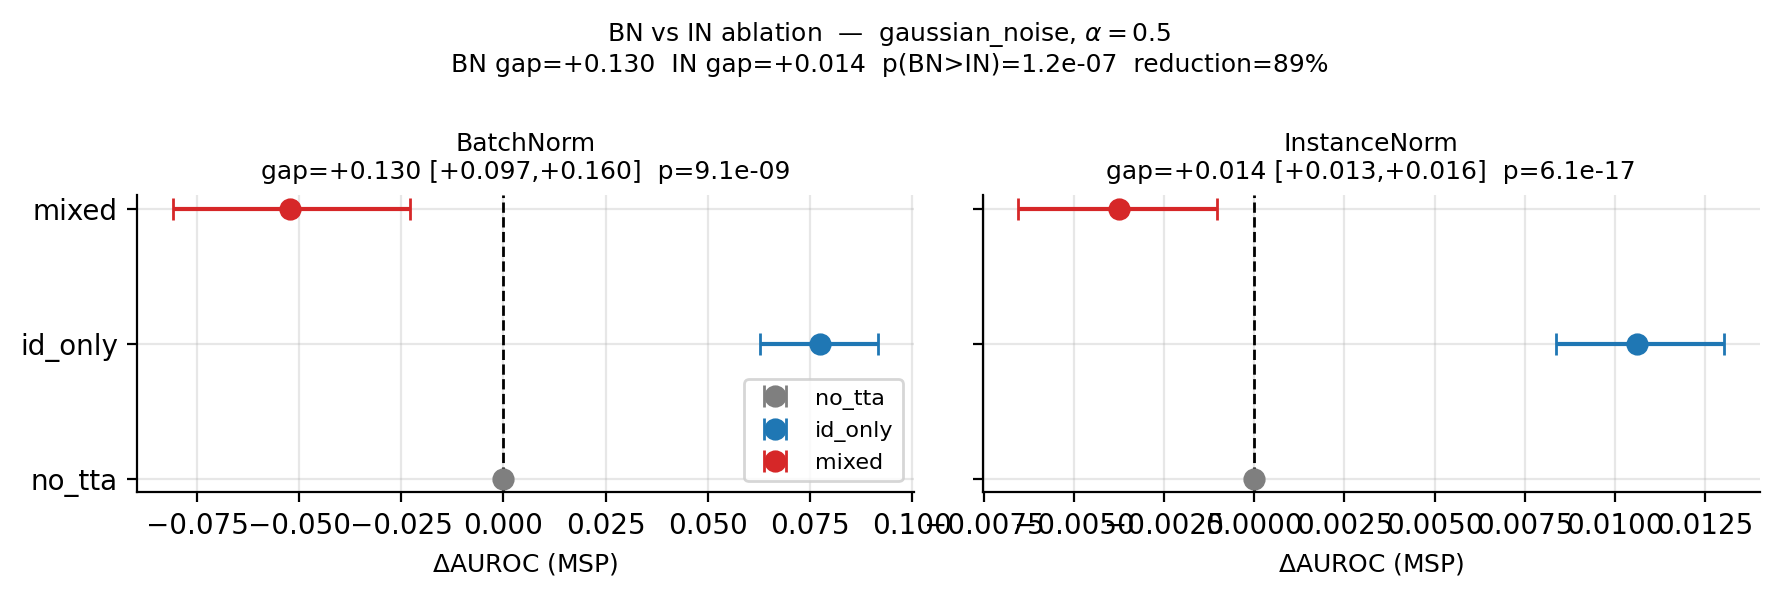
\includegraphics[width=0.6\linewidth]{figures/fig_ablation_bn.png}
  \caption{%
    BatchNorm vs.\ InstanceNorm ablation (SVHN, $\alpha=0.5$, gaussian noise).
    BN-TENT shows larger absolute gaps (both benefit and cost).
    IN-TENT shows a smaller absolute gap but similar forfeit fraction ($1.36$ vs.\ $1.67$).
    The reduction reflects weaker adaptation overall, not BN-statistics-specific contamination.
  }
  \label{fig:ablation_bn}
\end{figure}

\subsection{ViT-S/16 Backbone}

ViT-S/16 (LayerNorm, 98.80\% CIFAR-10 accuracy) shows a paired gap of $+0.013$ ($p = 2.6 \times 10^{-10}$, SVHN, $\alpha=0.5$, gaussian noise).
This exactly matches the ResNet-18/InstanceNorm residual of $+0.014$, providing convergent evidence that gradient contamination persists without shared batch statistics.

\subsection{Cross-Method Audit Full Results}

Full 32-cell audit results are available in the supplementary materials.
Results at $\alpha = 0.5$ show the same ranking reversal pattern as $\alpha = 0.9$, with smaller absolute gaps consistent with the scatter analysis (Section~\ref{sec:characterization}).

\subsection{Detector Breadth}

Additional results for Energy and Mahalanobis detectors across DTD and Places365 confirm that the paired gap is not specific to MSP.
For DTD $\alpha = 0.9$: Energy gap $= +0.225$ ($p = 1.7 \times 10^{-12}$); Mahalanobis gap $= +0.031$ ($p = 2.9 \times 10^{-4}$).

\section{Implementation Details}
\label{sec:appendix_impl}

\paragraph{TENT and ETA.}
Both methods adapt only the BatchNorm affine parameters ($\gamma, \beta$) using the Adam optimizer with $\text{lr} = 10^{-3}$.
BatchNorm layers are set to training mode with \texttt{track\_running\_stats=False}, so batch statistics are computed fresh from each test batch.
$T = 10$ gradient steps per batch.

\paragraph{UniEnt+.}
Implementation follows \citet{unient}: entropy split at $\tau = \log(C)/2$ where $C = 10$ for CIFAR-10.
Pseudo-ID samples ($H(p) < \tau$) receive entropy minimization loss; pseudo-OOD samples ($H(p) \ge \tau$) receive entropy maximization loss.
Same BatchNorm setup as TENT.

\paragraph{InstanceNorm ablation.}
BatchNorm layers are replaced by InstanceNorm using a deep-copy of the pretrained checkpoint, with affine parameters ($\gamma, \beta$) initialized from the original BN values.

\paragraph{ViT-S/16.}
The model is \texttt{vit\_small\_patch16\_224} from timm \citep{timm}, pretrained on ImageNet, fine-tuned 30 epochs on CIFAR-10 at $224 \times 224$.
LayerNorm affine parameters ($50$ pairs, $19.2k$ scalars) are adapted during TTA.

\paragraph{ImageNet-Scale.}
ResNet-50 torchvision pretrained weights ($\sim 76\%$ clean top-1).
NINCO \citep{ninco}: 5,878 images from 64 species not present in ImageNet-1K.
ImageNet-C \citep{imagenetc}: severity 5.
Batch size $64$, $T=20$ steps.

\paragraph{Statistical protocol.}
All confidence intervals use 1000-iteration bootstrap resampling (seed fixed per cell).
Paired $t$-test compares per-batch $\DeltaA$ vectors between conditions.
All $p$-values are two-sided.

\paragraph{Reproducibility.}
Code and checkpoints will be released at \texttt{[anonymous URL]}.
All experiments use \texttt{uv run python -m experiments.<script>}.
